% !Mode:: "TeX:UTF-8"
% !TEX root = ..\Literature_Translation.tex
\kchapter{计算实验}
在本章,将通过计算实验来评估MIP 模型和所提出的启发式算法的运行情况。
参考实际数据\reft{tab:2yearproduction},装配车间每月大约能装配24件作业,故实验可以通过3部分进行:\begin{inparaenum}[(1)]
\item 时间域为$2$周的包含$n=12$件作业的小型问题;
\item 时间域为$1\text{或}2.5$月的包含对应$n=24\text{或}n=60$件作业的中型问题;
\item 时间域为$4,8,12$月的包含对应$n=100,200,300$件作业的中型问题。
\end{inparaenum}
所有启发式方法皆用MATLAB 语言编写程序,并在处理器为AMD Athlon 2.91 GHz 的PC 上运行。
\ksection{评估小型问题}
我们随机产生10个12件作业和4个产品簇的示例($N=10$),其中$f_j$由均匀分布$DU(1,4)$产生,$d_j$由均匀分布$DU(100,180)$产生。
为了评估这些启发式方法的效果,考虑两个度量方面:求解质量和运行时间(Hamta,2012)。
为了检测启发式方法的求解质量,我们可以计算平均百分相对偏差(ARPD)如下(Laha 和Sarin,2009):
\[ARPD = \frac{100}{N}\sum_{i=1}^N\left(\frac{Heuristic_i - Optimal_i}{Optimal_i}\right)
\]
其中,$Heuristic_i$是第$i$个示例用启发式方法得到的目标函数值,$Optimal_i$是其MIP 目标函数值。
我们计算3个启发式方法EDD,FBEDD 和FBFS 按$(\alpha,\beta,\gamma)=(n/2,2,2)=(12/2,2,2)=(0.6,0.2,0.2)$加权的目标函数值和ARPD 的结果如\reft{tab:comparisonforarpd}所示。
\begin{table}[h]
  \centering\xiaowu
  \caption{MIP 和3个启发式方法的ARPD 比较\label{tab:comparisonforarpd}}
    \begin{tabular}{ccccccccc}
    \toprule
    \multirow{2}[4]{*}{示例编号} & \multicolumn{2}{c}{MIP} & \multicolumn{2}{c}{EDD} & \multicolumn{2}{c}{FBEDD} & \multicolumn{2}{c}{FBFS} \\
   \cmidrule(lr){2-3}\cmidrule(lr){4-5}\cmidrule(lr){6-7}\cmidrule(lr){8-9}
          & Z     & time(s) & Z     & ARPD  & Z     & ARPD  & Z     & ARPD \\
      \midrule
    1     & 331.04 & 10    & 423.64 & 27.97 & 375.92 & 13.56 & 331.04 & 0 \\
    2     & 374.56 & 15    & 435.88 & 16.37 & 396.88 & 5.96  & 376.48 & 0.51 \\
    3     & 338.72 & 21    & 425.64 & 25.66 & 380.08 & 12.21 & 344.48 & 1.7 \\
    4     & 332.4 & 123   & 399.48 & 20.18 & 354.32 & 6.59  & 338.16 & 1.73 \\
    5     & 377.28 & 35    & 435.84 & 15.52 & 395.2 & 4.75  & 377.28 & 0 \\
    6     & 342.64 & 47    & 441.2 & 28.76 & 393.68 & 14.9  & 342.64 & 0 \\
    7     & 316.64 & 24    & 414.64 & 30.95 & 349.64 & 10.42 & 316.64 & 0 \\
    8     & 345.36 & 22    & 443.28 & 28.35 & 391.48 & 13.35 & 345.36 & 0 \\
    9     & 359.04 & 35    & 451.04 & 25.62 & 399.44 & 11.25 & 359.04 & 0 \\
    10    & 386.72 & 8     & 442.56 & 14.44 & 432.8 & 11.92 & 389.04 & 0.6 \\[3pt]
    平均值   & 350.44 & 34    & 431.32 & 23.38 & 386.94 & 10.49 & 352.02 & 0.45 \\
    \bottomrule
    \end{tabular}
\end{table}
由最后一行各ARPD 可以看出,EDD 为$23.38\%$,在区间$(14.44,30.95)\%$中,FBEDD 为$10.49\%$,在区间$(4.75,14.90)\%$中,而FBFS 仅为$0.45\%$,在区间$(0,1.73)\%$中,较其他两者小,因此,FBFS 的运行效果要明显优于其他两个。
至于运行时间,MIP 每次需要$34\ s$,在区间$(8,123)\ s$中,而FBEDD 和FBFS 皆只需小于$0.3\ s$。综上所述,FBFS 是针对小型问题的好方法。
\ksection{评估中、大型问题}
考虑紧急插单的情况,设计成由$80\%$的MTO(面向订单生产)作业和$20\%$的MTS(面向库存生产)作业组成的中、大型问题。我们将最短交付期$D_j$设置成至少15天($15\times 8 = 120\ h$),最长交付期设置成1年($365\times 8 = 3000\ h$),所以,交付期期间为$[120,3000]\ h$。
工期$d_j$的确定基于交付期和能力限制,正常工期($d_j = D_j$)设置成基于普通能力,紧张工期($d_j = D_j - 40$)和松弛工期($d_j = D_j$)设置成基于稀缺和宽裕能力。

由于这个问题是NP 困难,我们不能在可接受的时间内找到中、大型问题的最优解。
为了评估启发式方法的求解质量,我们用相对误差(RER)来比较启发式方法和下界的差。进一步说,我们定义相对改善率(RIR)来比较启发式方法和现行方法的运行差异(Mokhtari,2010)。
\[RIR(\%) = \frac{100}{N}\sum_{i=1}^N \left(\frac{Heuristic_i - Best_i}{Best_i}\right)
\]
其中,$Heuristic_i$是用启发式方法的第$i$个示例的求解值,$Best_i$是示例中的最优值。

对于中、大型问题,需要测试15类问题、5类作业($n = 24,60,100,200,300$)和3个水准的工期(紧张(T),正常(N),松弛(L))的组合。
每一个问题都包含10个示例,其中$f_j$由$DU(1,4)$产生,对于5类作业,$D_j$分别由$DU(120,360),DU(120,270),DU(120,1120),DU(120,2120),DU(120,3000)$产生。
我们用3种启发式方法计算$n=24,d_j=D_j$,及权重为$(\alpha,\beta,\gamma)=(n/2,2,2)=(24/2,2,2)=(0.75,0.125,0.125)$的问题的下界和目标值,汇总RER 和RIR 见\reft{tab:comparen=24}。
\begin{table}[h]
  \centering\xiaowu
  \caption{通过10个示例比较$n=24, d_j = D_j$问题的三种启发式方法\label{tab:comparen=24}}
    \begin{tabular}{cccccccccc}
    \toprule
    \multirow{2}[4]{*}{示例编号} & \multirow{2}[4]{*}{LB}   & \multicolumn{3}{c}{目标值(Z)} & \multicolumn{3}{c}{RER (\%)} & \multicolumn{2}{c}{RIR (\%)} \\
    \cmidrule(lr){3-5}\cmidrule(lr){6-8}\cmidrule(lr){9-10}
          &       & (1) EDD & (2) FBEDD & (3) RFBFS &\parbox[c][8mm]{0pt}{} $\frac{(1) - LB}{LB}$ & $\frac{(2) - LB}{LB}$ & $\frac{(3) - LB}{LB}$ &$\frac{(1) - (3)}{(3)}$ & $\frac{(2) - (3)}{(3)}$ \\
          \midrule 
    1     & 661.5 & 953.4 & 748.9 & 698.9 & 44.13 & 13.22 & 5.66  & 36.41 & 7.15 \\
    2     & 723.3 & 1047.6 & 824.2 & 744.4 & 44.84 & 13.95 & 2.92  & 40.73 & 10.72 \\
    3     & 723.2 & 998.2 & 825.3 & 765.8 & 38.02 & 14.11 & 5.88  & 30.35 & 7.77 \\
    4     & 722.7 & 956.5 & 811.6 & 743.5 & 32.36 & 12.31 & 2.88  & 28.66 & 9.17 \\
    5     & 762.2 & 1029.9 & 898.9 & 808.5 & 35.12 & 17.94 & 6.07  & 27.38 & 11.18 \\
    6     & 661.2 & 918.9 & 733.4 & 683.9 & 38.98 & 10.92 & 3.43  & 34.37 & 7.24 \\
    7     & 761.1 & 963.3 & 846.8 & 791.3 & 26.58 & 11.26 & 3.97  & 21.74 & 7.01 \\
    8     & 732.8 & 997.7 & 850.3 & 790.6 & 36.15 & 16.03 & 7.89  & 26.19 & 7.54 \\
    9     & 748.4 & 934   & 830.9 & 791.3 & 24.8  & 11.03 & 5.73  & 18.03 & 5.01 \\
    10    & 663.9 & 934.8 & 742   & 709.9 & 40.8  & 11.76 & 6.92  & 31.68 & 4.53 \\[3pt]
    平均值   & 716   & 973.4 & 811.2 & 752.8 & 35.95 & 13.3  & 5.14  & 29.31 & 7.76 \\
    \bottomrule
    \end{tabular}
\end{table}
由最后一行可以看出,EDD 和FBEDD 分别有平均RER $35.95\%\text{和}13.30\%$,而RFBFS 为$5.14\%$。同时可以看出,RFBFS 比EDD 和FBEDD 好,因为两者的平均RIR 分别为$29.31\%\text{和}7.76\%$。因此,RFBFS 就求解质量将提高效果上来说要优于其余两者。

我们用同样的方法计算目标值函数、RER 和RIR,所有组合的权重为$(\alpha,\beta,\gamma) = (n/2,2,2)$。结果的平均值汇总在\reft{tab:allcompare},
\begin{table}[h]
  \centering\xiaowu
  \caption{所有组合的三种启发式方法比较\label{tab:allcompare}}
    \begin{tabular}{crccccccccc}
    \toprule
    \multirow{2}[4]{*}{n} & \multicolumn{1}{c}{\multirow{2}[4]{*}{$d_j$}} & \multirow{2}[4]{*}{LB} & \multicolumn{3}{c}{目标函数值 (Z)} & \multicolumn{3}{c}{RER (\%)} & \multicolumn{2}{c}{RIR (\%)} \\
    \cmidrule(lr){4-6}\cmidrule(lr){7-9}\cmidrule(lr){10-11}
          & \multicolumn{1}{c}{} &       & (1) EDD & (2) FBEDD & (3) RFBFS &\parbox[c][8mm]{0pt}{} $\frac{(1) - LB}{LB}$ & $\frac{(2) - LB}{LB}$ & $\frac{(3) - LB}{LB}$ &$\frac{(1) - (3)}{(3)}$ & $\frac{(2) - (3)}{(3)}$\\
      \midrule    
    \multirow{3}[1]{*}{24} & T     & 743   & 1017  & 824   & 769   & 36.77 & 10.92 & 3.48  & 32.17 & 7.19 \\
          & N     & 716   & 973   & 811   & 753   & 35.95 & 13.3  & 5.14  & 29.31 & 7.76 \\
          & L     & 701   & 957   & 811   & 753   & 36.59 & 15.78 & 7.42  & 27.15 & 7.78 \\[3pt]
    \multirow{3}[0]{*}{60} & T     & 2036  & 2892  & 2339  & 2156  & 42.08 & 14.91 & 5.92  & 34.14 & 8.49 \\
          & N     & 1977  & 2802  & 2268  & 2094  & 41.71 & 14.7  & 5.91  & 33.8  & 8.3 \\
          & L     & 1931  & 2735  & 2221  & 2054  & 41.65 & 15.04 & 6.38  & 33.15 & 8.14 \\[3pt]
    \multirow{3}[0]{*}{100} & T     & 3537  & 5170  & 4144  & 3774  & 46.18 & 17.16 & 6.71  & 36.99 & 9.79 \\
          & N     & 3468  & 5050  & 4045  & 3702  & 45.61 & 16.64 & 6.76  & 36.4  & 9.26 \\
          & L     & 3403  & 4939  & 3939  & 3633  & 45.16 & 15.77 & 6.79  & 35.93 & 8.41 \\[3pt]
    \multirow{3}[0]{*}{200} & T     & 7208  & 10,552 & 8301  & 7662  & 46.39 & 15.17 & 6.3   & 37.71 & 8.34 \\
          & N     & 7141  & 10,412 & 8169  & 7592  & 45.8  & 14.39 & 6.31  & 37.14 & 7.59 \\
          & L     & 7077  & 10,278 & 8044  & 7524  & 45.22 & 13.66 & 6.31  & 36.59 & 6.91 \\[3pt]
    \multirow{3}[1]{*}{300} & T     & 10,817 & 15,844 & 12,338 & 11,487 & 46.47 & 14.06 & 6.19  & 37.93 & 7.41 \\
          & N     & 10,753 & 15,697 & 12,196 & 11,418 & 45.98 & 13.42 & 6.19  & 37.48 & 6.81 \\
          & L     & 10,690 & 15,555 & 12,060 & 11,350 & 45.51 & 12.82 & 6.17  & 37.05 & 6.26 \\
    \bottomrule
    \end{tabular}
\end{table}
可以看出,EDD 和FBEDD 的平均RER 分别为$35.95\% - 46.47\%$和$10.92\% - 17.16\%$,而RFBFS 为$3.48\% - 7.42\%$,要明显优于前两者。
同时,可以发现其平均RIR 和RFBFS 也要明显优于EDD h($27.15\% - 37.93\%$)和FBEDD$6.29\% - 9.79\%$。因此,可以得出结论:RFBFS 表现要优于EDD
 和FBEDD。
这些反映了完整批和簇分类的特性,对该问题有正面影响,并且影响会随问题型号增大而加强。
此外,我们注意到几乎所有的问题会随工期的紧迫程度增加而得到更好的RER 和RIR。这就表示,严格控制工期可以改善调度效果。

在前面的实验中,我们假设只有4个簇($f=4$)以简化问题。为了验证RFBFS 可运用到其他情形,需要设计更多实验。我们修改$n=24$,作业簇为18,19,20的示例,对于$f = 5$将其改为$f_j=5$;作业簇为15,16,17的示例,对于$f = 6$将其改为$f_j=6$,结果汇总于\reft{tab:n=24compare},
\begin{table}[h]
  \centering\xiaowu
  \caption{对于$n=24$时不同产品簇的3种启发式方法的比较\label{tab:n=24compare}}
    \begin{tabular}{ccccccccccc}
    \toprule
    \multirow{2}[4]{*}{$f$} & \multirow{2}[4]{*}{$d_j$} & \multirow{2}[4]{*}{LB} & \multicolumn{3}{c}{目标函数值 (Z)} & \multicolumn{3}{c}{RER (\%)} & \multicolumn{2}{c}{RIR (\%)} \\
    \cmidrule(lr){4-6}\cmidrule(lr){7-9}\cmidrule(lr){10-11}
          &       &       & (1) EDD & (2) FBEDD & (3) RFBFS & $\frac{(1) - LB}{LB}$ & $\frac{(2) - LB}{LB}$ &\parbox[c][8mm]{0pt}{}  $\frac{(3) - LB}{LB}$ &$\frac{(1) - (3)}{(3)}$ & $\frac{(2) - (3)}{(3)}$\\
          \midrule
    \multirow{3}[1]{*}{4} & T     & 743   & 1017  & 824   & 769   & 36.77 & 10.92 & 3.48  & 32.17 & 7.19 \\
          & N     & 716   & 973   & 811   & 753   & 35.95 & 13.3  & 5.14  & 29.31 & 7.76 \\
          & L     & 701   & 957   & 811   & 753   & 36.59 & 15.78 & 7.42  & 27.15 & 7.78 \\[3pt]
    \multirow{3}[0]{*}{5} & T     & 740   & 1040  & 844   & 780   & 40.48 & 14    & 5.34  & 33.36 & 8.22 \\
          & N     & 714   & 985   & 819   & 760   & 37.93 & 14.71 & 6.3   & 29.76 & 7.92 \\
          & L     & 698   & 967   & 813   & 756   & 38.55 & 16.58 & 8.38  & 27.84 & 7.56 \\[3pt]
    \multirow{3}[1]{*}{6} & T     & 737   & 1057  & 855   & 787   & 43.49 & 16.13 & 6.85  & 34.29 & 8.68 \\
          & N     & 713   & 1000  & 829   & 769   & 40.19 & 16.31 & 7.81  & 30.04 & 7.88 \\
          & L     & 696   & 978   & 821   & 762   & 40.53 & 18.02 & 9.54  & 28.29 & 7.74 \\
    \bottomrule
    \end{tabular}
\end{table}
可以看到,EDD 和FBEDD 求解的平均RER 分别为$35.95\% - 43.49\%$和$10.92\% - 18.02\%$,而RFBFS 为$3.48\% - 9.54\%$。同时,可以发现RFBFS 的平均RIR 为$7.19\% - 8.68\%$,比FBEDD($27.15\% - 34.29\%$)高,也比EDD 高。
由此可得,RFBFS 的在求解质量、评测改善上表现优于EDD 和FBEDD,而且两者皆随作业簇的数量增加而轻微提高。
\ksection{实际表现评估}
为了进一步验证所提调度方法的运行情况,我们根据2.5节所提的3个问题提供了3个运行标准,包括短缺时间、流程时间和准时完成率。
我们收集了从2009年1月到6月的车间一线数据,并比较了他们使用所提方法前后的运行情况,结果见\reft{tab:performancemeasure}和\reff{fig:performancemeasures}(横坐标皆为周期),
\begin{table}[h]
  \centering\xiaowu
  \caption{车间运行测评\label{tab:performancemeasure}}
    \begin{tabular}{ccccc}
    \toprule
    周期 (月) & 作业数量  & 平均短缺时间 (h) & 平均流程时间 (h) & 准时完成率 \\
    \midrule
    0     & 24    & 2.67  & 228   & 0.15 \\
    1     & 12    & 1.17  & 128   & 0.5 \\
    2     & 12    & 1     & 121   & 0.6 \\
    3     & 16    & 0.63  & 160   & 0.65 \\
    4     & 16    & 0.75  & 158   & 0.78 \\
    5     & 24    & 0.75  & 194   & 0.82 \\
    6     & 24    & 0.71  & 188   & 0.86 \\
    \bottomrule
    \end{tabular}
\end{table}\vspace{-0.8cm}
\begin{figure}[h]
\begin{floatrow}
  \subfloat[平均短缺时间(h) \label{fig:starvation}]{\centering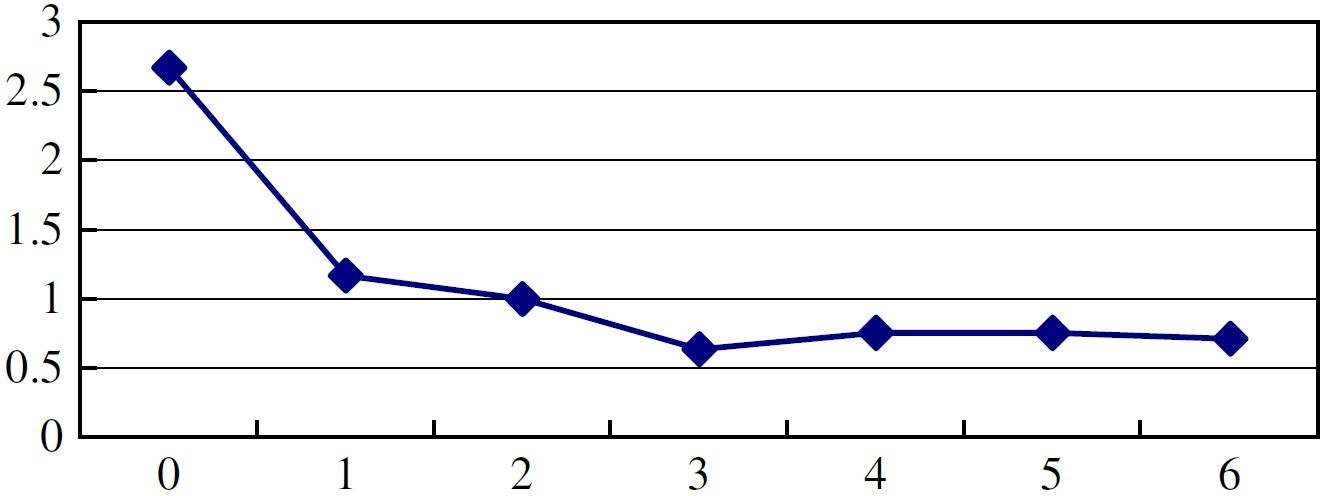
\includegraphics[width=5cm,height=2cm]{starvationtime.jpg}}
  \subfloat[平均流程时间(h) \label{fig:flow}]      {\centering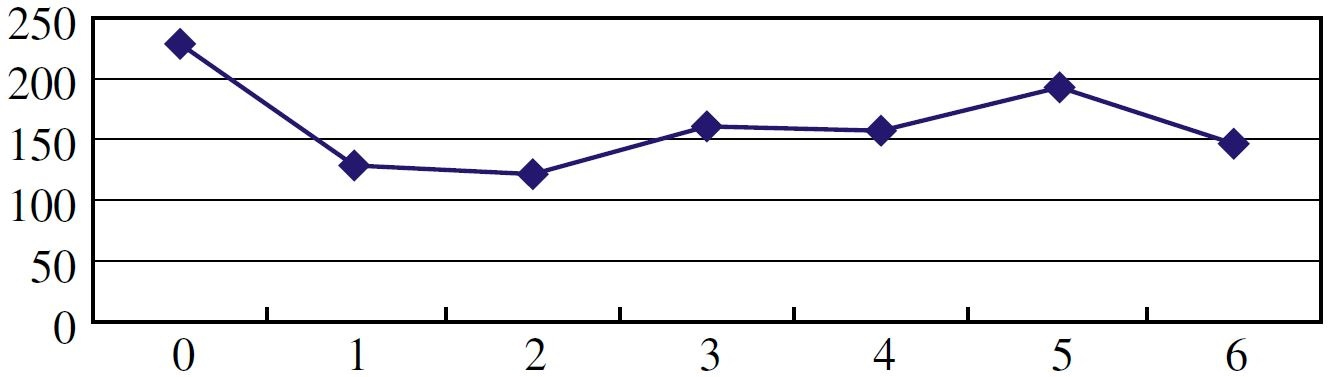
\includegraphics[width=5cm,height=2cm,trim = 30 0 0 0]{flowtime.jpg}}
  \subfloat[准时完成率\label{fig:ontime}]          {\centering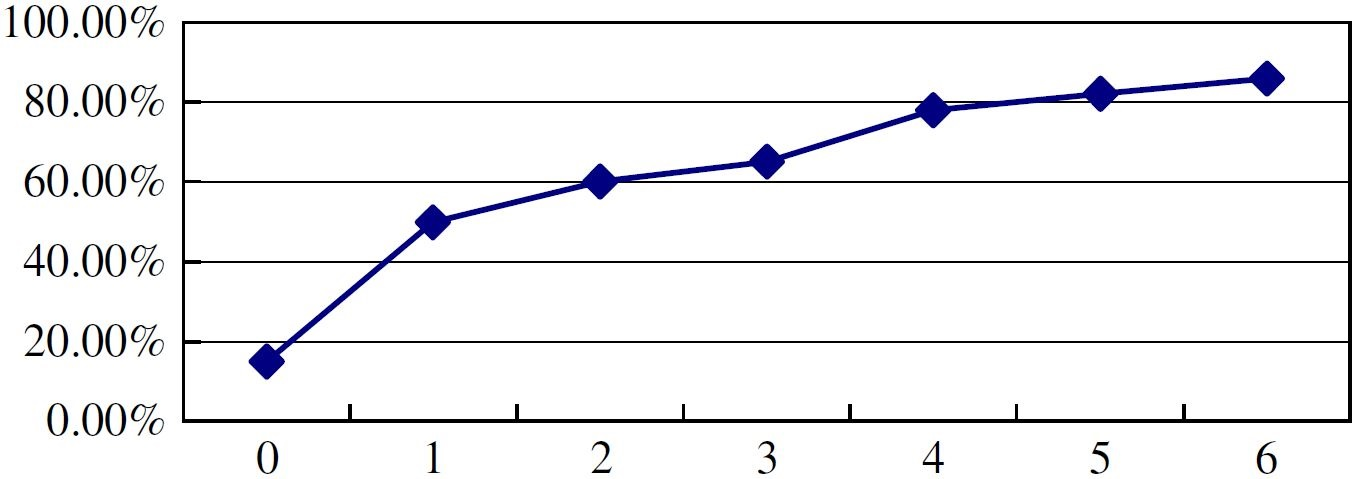
\includegraphics[width=5cm,height=2cm,trim = -20 0 0 0]{ontimerate.jpg}}
  \caption{车间运行评估\label{fig:performancemeasures}}
  \end{floatrow}
\end{figure}
其中周期0表示使用方法前的测量值。可以发现用了批量处理后短缺时间显著减少,同时,用了作业划分和簇调度后,流程时间和准时完成率显著提高。